%set the master document for easy compilation
%!TEX root = ../D3_5_2.tex

\section{Manage\_Radio\_Communication}

\subsection{Component Requirements}

\begin{longtable}{p{.25\textwidth}p{.7\textwidth}}
\toprule
Component name			& Mode\_and\_Level \\
\midrule
Link to SCADE model		& {\footnotesize \url{???}} \\
\midrule
SCADE designer			& Uwe Steinke, Siemens AG \\
\midrule
Description				& ??? \\
\midrule
Input documents	& 
Subset-026, Chapter 4 \newline
Subset-026, Chapter 5 \\
\midrule
Safety integrity level	& 4 \\
\midrule
Time constraints		& [If applicable description of time constraints, otherwise n/a] \\
\midrule
API requirements 		& [If applicable description of API requirements, otherwise n/a] \\
\bottomrule
\end{longtable}


\subsection{Interface}

An overview of the interface of component Mode\_and\_Level is shown in Figure~\ref{f:manage_radio_communication_interface}. The inputs and outputs are described in detail in Section~\ref{s:manage_radio_communication_inputs} respectively \ref{s:manage_radio_communication_outputs}.

\begin{figure}
\center
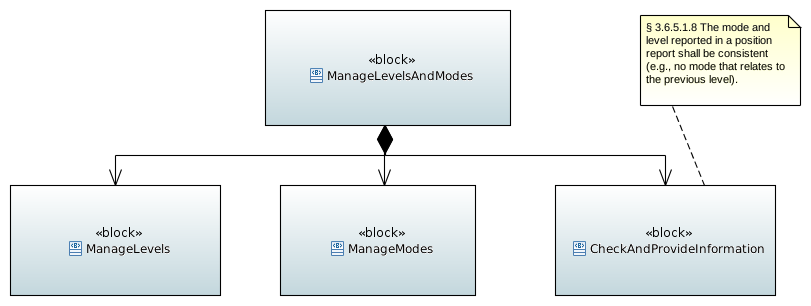
\includegraphics[width=\textwidth]{images/FunctionalArchitecture.png}
\caption{Component SysML diagram}\label{f:manage_radio_communication_interface}
\end{figure}


\subsubsection{Inputs}\label{s:manage_radio_communication_inputs}

\paragraph{[Input 1 name]}

\begin{longtable}{p{.25\textwidth}p{.7\textwidth}}
\toprule
Input name				& [Name of the input] \\
\midrule
Description				& [Brief description of the input] \\
\midrule
Source					& [Name of the source component] \\ 
\midrule
Type					& [Type of the input] \\
\midrule
Valid range of values	& [Complete list of valid values] \\
\midrule
Behaviour when value is at boundary	& [Description of components behaviour when input value is at boundary] \\
\midrule
Behaviour for values out of valid range	& [Description of components behaviour when input value is out of valid range] \\
\bottomrule
\end{longtable}


\paragraph{[Input 2 name]}

\begin{longtable}{p{.25\textwidth}p{.7\textwidth}}
\toprule
Input name				& [Name of the input] \\
\midrule
Description				& [Brief description of the input] \\
\midrule
Source					& [Name of the source component] \\ 
\midrule
Type					& [Type of the input] \\
\midrule
Valid range of values	& [Complete list of valid values] \\
\midrule
Behaviour when value is at boundary	& [Description of components behaviour when input value is at boundary] \\
\midrule
Behaviour for values out of valid range	& [Description of components behaviour when input value is out of valid range] \\
\bottomrule
\end{longtable}


\subsubsection{Outputs}\label{s:manage_radio_communication_outputs}

\paragraph{[Output 1 name]}

\begin{longtable}{p{.25\textwidth}p{.7\textwidth}}
\toprule
Output name				& [Name of the output] \\
\midrule
Description				& [Brief description of the output] \\
\midrule
Destination				& [Name of the destination component(s)] \\ 
\midrule
Type					& [Type of the output] \\
\midrule
Valid range of values	& [Complete list of valid values] \\
\midrule
Behaviour when value is at boundary	& [Description of components behaviour when output value is at boundary] \\
\midrule
Behaviour for values out of valid range	& [Description of components behaviour when output value is out of valid range] \\
\bottomrule
\end{longtable}


\paragraph{[Output 2 name]}

\begin{longtable}{p{.25\textwidth}p{.7\textwidth}}
\toprule
Output name				& [Name of the output] \\
\midrule
Description				& [Brief description of the output] \\
\midrule
Destination				& [Name of the destination component(s)] \\ 
\midrule
Type					& [Type of the output] \\
\midrule
Valid range of values	& [Complete list of valid values] \\
\midrule
Behaviour when value is at boundary	& [Description of components behaviour when output value is at boundary] \\
\midrule
Behaviour for values out of valid range	& [Description of components behaviour when output value is out of valid range] \\
\bottomrule
\end{longtable}


\subsection{Sub Components}

\subsubsection{Management\_of\_Radio\_Communication}
%set the master document for easy compilation
%!TEX root = ../D3_5_3.tex

\paragraph{Component Requirements}

\begin{longtable}{p{.25\textwidth}p{.7\textwidth}}
\toprule
Component name			& MoRC\_Main\_v2 (Management\_of\_Radio\_Communication) \\
\midrule
Link to SCADE model		& {\footnotesize \url{https://github.com/openETCS/modeling/tree/master/model/Scade/System/ObuFunctions/Radio/MoRC}} \\
\midrule
SCADE designer			& Uwe Steinke, Siemens \\
\midrule
Description				& 
The function \emph{MoRC\_Main\_v2} implements the session states establishing, maintaining and terminating as described in Subset-026, chap. 3.5. A SCADE state machine reflects this state model  accurately. Within each of the states, the activities needed as long as the state is active, are performed. \newline

\emph{MoRC\_Main\_v2} is related to exactly one of the radio mobile modems onboard, monitors its status and controls the processes of registration to the radio network, connecting to one RBC and establishing a radio session with the RBC. \emph{MoRC\_Main\_v2} communicates with its mobile modem directly via the API.  \newline

As the OBU is required to manage up to two RBCs,  two instances of \emph{MoRC\_Main\_v2} are used.  \newline

In addition, \emph{MoRC\_Main\_v2} generates the radio connection indication for the driver.

\\
\midrule
Input documents	& 
Subset-026, Chapter 3.5 \\
\midrule
Safety integrity level		& 4 \\
\midrule
Time constraints		& Implements several time delays, therefore appropriate clocking required \\
\midrule
API requirements 		& Interfaces to the OBUs mobile modem hardware via API \\
\bottomrule
\end{longtable}


\paragraph{Interface}

For an overview of the interface of this internal component we refer to the SCADE model (cf.~link above) respectively the SCADE generated documentation.


